% le titre donné dans la lettre terminait par: «avec un focus sur la
% recherche du partenaire supersymmétrique du gluon, le gluino, se
% désintégrant en quarks top »
\singlespacing{}
\chapter{La recherche de la Supersymétrie à ATLAS}
\label{sec:susy_atlas}
\doublespacing{}

% Intro: rappel motivations SUSY
Comme vu dans le chapitre~\ref{sec:susy}, une extension
supersymétrique minimale du Modèle Standard permettrait de
simultanément régler le problème de la hiérarchie des masses,
d'expliquer la nature de la matière sombre et d'unifier tous les
couplages. De plus, certaines des nouvelles particules prédite par la
supersymétrie pourraient avoir des masses de l'ordre du TeV, ce qui
signifie qu'il serait possible de les créer lors de collisions
proton-proton au LHC. Conséquemment, la collaboration ATLAS recherche
activement des manifestations des superpartenaires depuis le début du
programme de physique au LHC~\cite{aad_summary_2015}. 

Les signatures expérimentales typiques des processus supersymétriques
sont présentés dans la section~\ref{sec:susy_atlas:signatures}. Une
recherche de gluinos se désintégrant en tops est ensuite résumée dans
la section~\ref{sec:susy_atlas:gtt} et la
section~\ref{sec:susy_atlas:dl} termine le chapitre en traitant de
l'utilisation possible des techniques d'apprentissage machine dans le
cadre de recherches de physique au-delà du Modèle Standard.

\section{Signatures expérimentales}
\label{sec:susy_atlas:signatures}

% Mécanismes de production
Parmi les processus supersymétriques possibles, les productions de
paires squark-squark, gluino-gluino ou squark-gluino ont des sections
efficaces très élevées au LHC~\cite{olive_susy2_2014}, comme le montre
la figure~\ref{fig:susy_xsec}.

\begin{figure}
  \centering
  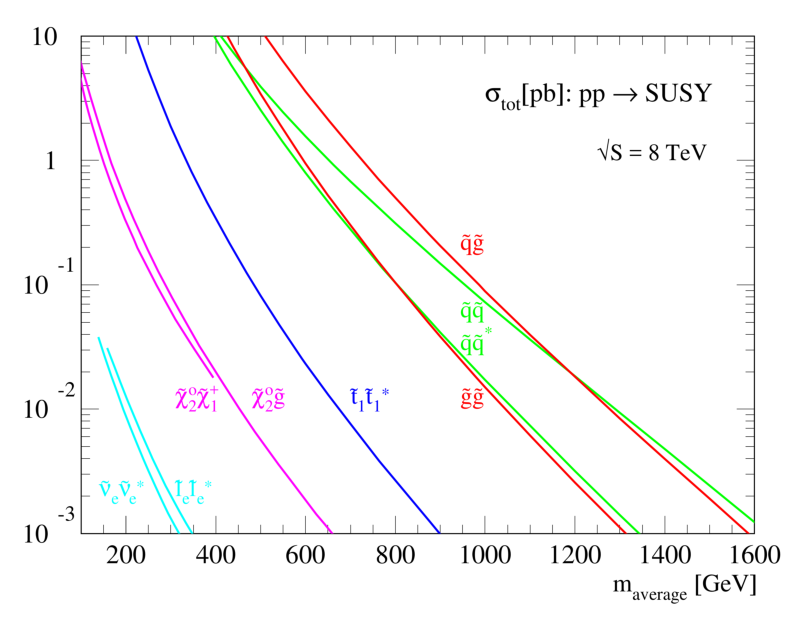
\includegraphics[width=.5\textwidth]{susy_xsec.pdf}
  \caption{Sections efficaces de production de paires de particules
    supersymétriques en fonction de la masse. Le symbole $\tilde{q}$
    représente tous les squarks sauf le stop. Figure tirée de la
    référence~\cite{olive_susy2_2014}.}
  \label{fig:susy_xsec}
\end{figure}

Puisque les gluinos et les squarks pourraient avoir une masse de
l'ordre du TeV, donc beaucoup plus élevé que les masses des particules
du Modèle Standard dans lesquelles ils se désintègrent, les processus
supersymétriques sont souvent caractérisés par la présence de
plusieurs gerbes de très haute impulsion. En outre, puisque
l'impulsion transverse des protons initiaux ainsi que de leur
constituant peut être négligée, La somme vectorielle de l'impulsion
transverse de toutes les particules produites lors d'une interaction
devrait être nulle, par la conservation de l'impulsion. Or, certaines
particules comme les neutrinos ne sont pas détectés ce qui engendre
une impulsion transverse manquante, noté $\slashed{E}_T$. Assumant la
conservation de la R-parité~(section~\ref{sec:susy:R}), il va toujours
y avoir une paire de LSP stables dans l'état final d'une
cascade supersymétrique. Ces particules sont potentiellement neutres et
interagiraient donc seulement faiblement, traversant le détecteur sans
être dépistées. Une deuxième signature caractéristique d'un processus
supersymétrique est donc une $\slashed{E}_T$ très
élevée~\cite{olive_susy2_2014}.


\section{Recherche des gluinos se désintégrant en tops}
\label{sec:susy_atlas:gtt}

% C.F. chapitre précédent: haute section efficace pour decay with tops
Comme vu précédemment, les recherches de stops avec masses de l'ordre
du TeV au LHC sont bien motivées à cause du problème de la hiérarchie
des masses. La figure~\ref{fig:susy_xsec} montre cependant que la
section efficace de paires de stops est plus faible que, par exemple,
la section efficace gluino-gluino. Dans plusieurs réalisation du MSSM,
le gluino a un grand rapport d'embranchement pour les désintégrations
$\tilde{g} \rightarrow \tilde{t} t$~\cite{bandyopadhyay_boosted_2011}.
De plus, le gluino doit aussi avoir une masse de l'ordre du TeV pour
que le MSSM règle le problème de la hiérarchie des masses, ce qui
motive la recherche du stop dans le contexte de la production de
paires de gluinos.

Comme vu à la section~\ref{sec:top:boosted:susy}, ces processus
engendrent typiquement des états finaux avec haute multiplicité de
quarks top à haute impulsion transverse. Cette multiplicité est à un
maximum lorsque les deux gluinos se désintègrent en stop et en top et
que le stop se désintègre subséquemment en top et en neutralino, tel
qu'illustré dans la figure~\ref{fig:susy_feyn}. Ce processus fait l'objet
de plusieurs recherche à ATLAS, notamment dans la référence~\cite{ATLAS-CONF-2015-067}.

\begin{figure}[h]
  \centering
  \begin{subfigure}{.5\textwidth}
    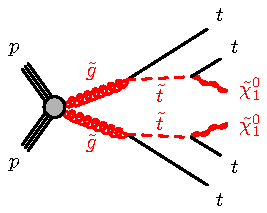
\includegraphics[width=\textwidth]{gogo-ttttN1N1-stst.pdf}
    \label{fig:sub1}
  \end{subfigure}%
  \begin{subfigure}{.5\textwidth}
    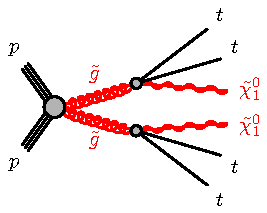
\includegraphics[width=\textwidth]{gogo-ttttN1N1.pdf}
    \label{fig:sub2}
  \end{subfigure}
  \caption{Diagrammes de Feynman pour la désintégration de paires de gluinos en stops et en tops avec stop
    réel~(gauche) ou virtuel~(droite).}
  \label{fig:susy_feyn}
\end{figure}
% Modèles simplifiés
% Description
% Stop off-shell
% commentaires sur l'état final 
% Montrer diagrammeS feynman

\subsection{Stratégie d'analyse}
\label{sec:susy_atlas:gtt:strategie}

La stratégie retenu dans la référence~\cite{ATLAS-CONF-2015-067} est
de séparer les événements où les tops se désintègrent hadroniquement et
semi-leptoniquement, définir quelques variables cinématiques dans ces
deux canaux ainsi que des seuils sur ces variables pour pouvoir
séparer les événements supersymétriques des événements du Modèle
Standard ayant une signature similaire (comme la production de paires
$t\overline{t}$) et de compter les événements passant ces seuils dans
les données enregistrés par le détecteur ATLAS. Le nombre d'événement
ainsi obtenu est comparé à la prédiction du modèle
standard pour déterminer s'il y a eu production de particules supersymétriques.

\noindent Les variables utilisés sont:

\begin{itemize}
\item $N_{gerbe}$, le nombre de gerbes hadroniques %avec impulsion $> 30$~GeV
\item $N_b$, le nombre de gerbes identifiés comme originant d'un quark $b$ (gerbes-$b$)
\item $N_{t}$, le nombre de gerbes identifiés comme originant d'un
  quark top, selon un discriminant basé sur la masse de la gerbe
\item $\slashed{E}_T$, tel que définie dans la
  section~\ref{sec:susy_atlas:signatures}
\item $m_T$, la masse transverse de $\slashed{E}_T$ et du lepton le
  plus énergétique
\item $m_{T,min}^b$, la masse transverse minimale de $\slashed{E}_T$ et
  d'une des gerbes-$b$
\item $m_{eff}$ la somme scalaire des impulsions des gerbes et des leptons, et de $\slashed{E}_T$.
\end{itemize}

Différents seuils sur ces variables définissent des \emph{régions de
  signal} dans lesquels le bruit de fond $t\overline{t}$ est fortement
supprimé. Les définitions des différentes régions se trouve dans la
référence~\cite{ATLAS-CONF-2015-067}.

% Par exemple, il y a deux régions de signal dans le canal
% semileptonique tel que résumé dans la table~\ref{tab:sr}.

% \begin{table}
%   \centering
%   \begin{tabular}{c|c|c}
%     \hline
%     Région & Variable & Seuil
%     \\ \hline \hline
%     \multirow{4}{*}{Commun}
%     & $m_T$ & 150 GeV \\ 
%     & $N_{gerbe}$ & 6 \\
%     & $N_b$ & 3 \\ \hline
%     & $m_{T,min}^b$ & 160 GeV \\ 
%     \multirow{3}{*}{1L-A}
%     & $\slashed{E}_T$ & 200 GeV \\ 
%     & $m_{eff}$ & 1100 GeV \\
%     & $N_{t}$ & 1 \\ \hline
%     \multirow{2}{*}{1L-B}
%     & $\slashed{E}_T$ & 300 GeV \\ 
%     & $m_{eff}$ & 900 GeV \\ \hline
%   \end{tabular}
% \caption{Régions de signal pour le canal leptonique de l'analyse~\cite{ATLAS-CONF-2015-067}.}
% \label{tab:sr}
% \end{table}

Des régions de contrôle riches en bruit de fond et pauvre en signal
sont définies en inversant certains seuils, et sont utilisés pour
estimer le montant de bruit de fond dans les données et en dériver un
facteur de correction pour les simulations Monte Carlo. Ces estimés sont ensuite
vérifiés dans des régions de validations, entre les régions de signal
et de contrôle. La figure~\ref{fig:pull} montre que l'estimation du
bruit de fond dans les régions de validation dans les simulations
Monte Carlo est en accord avec le bruit de fond observé dans les
collisions.

\begin{figure}
  \centering
  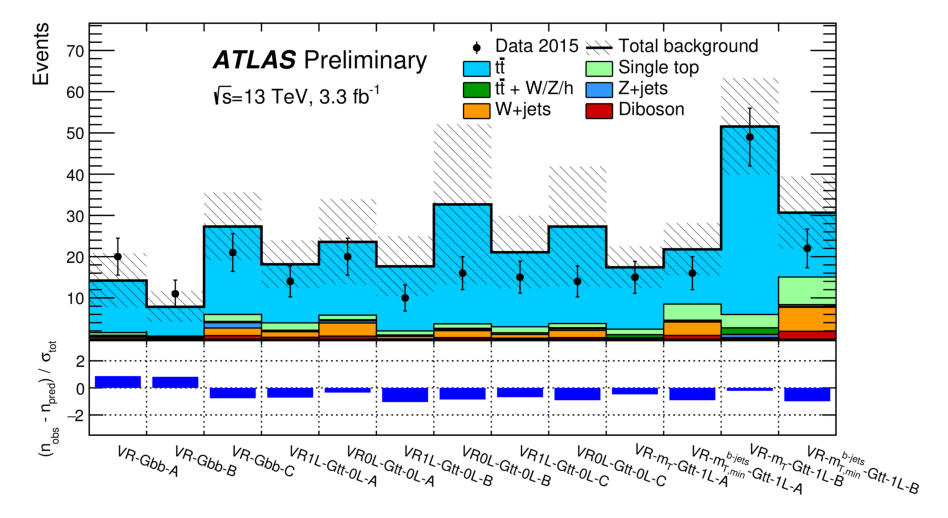
\includegraphics[width=.7\textwidth]{pull.pdf}
  \caption{Comparaison Monte Carlo vs données des nombres d'événements
    dans les régions de validation. Figure tirée de la
    référence~\cite{ATLAS-CONF-2015-067}}
\label{fig:pull}
\end{figure}

Aucun excès d'événement n'est observé dans les régions de signal.  Les
données sont donc utilisées pour fixer des limites inférieures sur les
masses des particules supersymétriques. La figure~\ref{fig:limit}
montre la limite dans le plan $m_{\tilde{g}}-m_{\chi_1^0}$ pour le
processus avec stop virtuel.

\begin{figure}[h!]
  \centering
  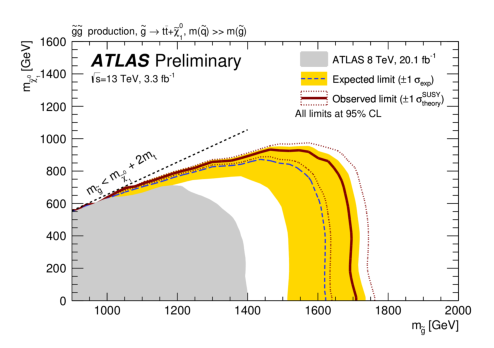
\includegraphics[width=.65\textwidth]{limit.pdf}
  \caption{Limites inférieures au niveau de confiance 95\% dans le
    plan $m_{\tilde{g}}-m_{\chi_1^0}$ dans le contexte de production
    de paires de gluinos se désintégrant en une paire de top et un
    neutralino via un stop virtuel.  Figure tirée de la
    référence~\cite{ATLAS-CONF-2015-067}}
  \label{fig:limit}
\end{figure}

\clearpage{}

\section{Recherches par apprentissage profond}
\label{sec:susy_atlas:dl}

% intro
Du fait du grand volume de données produites par le détecteur ATLAS et
des signaux difficiles à reconnaitres qui sont recherchés, il est très
important d'utiliser des approches statistiques à la fine pointe de la
technologie dans le cadre de recherches de nouvelles physique au
LHC. Une avenue future possible est de prendre avantage du
développement récent de techniques d'\emph{apprentissage
  profond}~\footnote{De l'anglais, \emph{Deep
    Learning}}~\cite{lecun_deep_2015, schmidhuber_deep_2015} ayant
récemment fait grand bruit en informatique à cause de leur performance
phénoménale mais dont l'utilisation en physique des particules reste
marginale.
 
\subsection{L'apprentissage machine}
\label{sec:susy_atlas:dl:ml}

L'apprentissage machine est un champ de recherche dans lequel sont
développé des modèles statistiques adaptatifs ainsi que des techniques
pour ajuster leurs paramètres automatiquement à partir
d'ensembles de données.

Un des modèle les plus performant est celui du \emph{réseau de
  neurones}. L'unité de base de ce modèle est la neurone, qui est un
une somme pondéré des variables d'entrée subséquemment transformée
non-linéairement,
\begin{eqnarray}
  y_j(\overrightarrow{x}) = h\left(\sum_jw_{ij}x_j + b_i\right)
\end{eqnarray}

\noindent où la fonction $h$ est une fonction non-linéaire. Plusieurs
de ces neurones peuvent être arrangés en réseau, produisant un modèle
très expressif dont on peut ajuster les poids pour approximer la fonction voulu.
La figure~\ref{fig:nn} montre une représentation graphique d'un tel
réseau de neurone.

\begin{figure}[h]
  \centering
  \begin{subfigure}{.5\textwidth}
    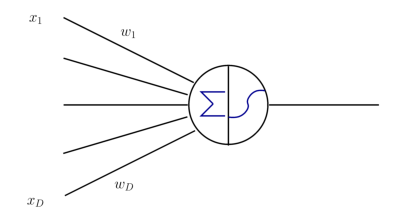
\includegraphics[width=\textwidth]{neuron.pdf}
    \label{fig:sub1}
  \end{subfigure}%
  \begin{subfigure}{.5\textwidth}
    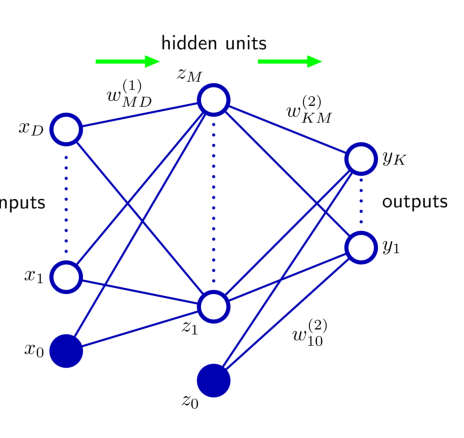
\includegraphics[width=\textwidth]{NN.pdf}
    \label{fig:sub2}
  \end{subfigure}
  \caption{Neurone (gauche) et réseau de neurone (droite). Figure tirée de la référence~\cite{bishop_pattern_2006}}
  \label{fig:nn}
\end{figure}

Le théorème d'approximation universelle stipule qu'un réseau de
neurone à une couche avec un nombre inconnu mais fini de neurones
peut approximer n'importe quelle fonction
continue~\cite{hornik_approximation_1991}. Or, les réseaux à plusieurs
couches sont \emph{exponentiellement} plus efficaces que les réseaux à
une couche, mais était considéré jusqu'à tout récemment comme très
difficiles à optimiser. Il existe cependant depuis quelques années
plusieurs techniques pour entraîner des modèles profond étant capable
d'approximer efficacement des fonctions de classification à partir de
données brutes~\cite{lecun_deep_2015}.

\subsection{Discrimination signal/bruit de fond}
\label{sec:susy_atlas:dl:evt}

L'application de techniques d'apprentissage profond pour estimer la
probabilité qu'un événement provienne d'un processus signal donné a
été explorée dans les références~\cite{baldi_enhanced_2015} et~\cite{baldi_searching_2014}.

Comme vu dans la section~\ref{sec:susy_atlas:gtt}, la technique typique de discrimination
signal/bruit de fond consiste à élaborer des variables physiques qui
encapsulent certaines caractéristiques du signal recherché. La
puissance des modèles d'apprentissage profond permet cependant
d'utiliser directement des quantités de plus bas niveau, comme par
exemple les quadri-impulsions des gerbes. Ces modèles sont capable d'utiliser
ces variables pour obtenir un pouvoir de discrimination plus élevé que
celui des variables de haut niveau élaborés par les physiciens, tel
qu'illustré dans la figure~\ref{fig:deep} pour un signal
$Higgs \rightarrow\tau\tau$.  Dans cette figure, tirée de la
référence~\cite{baldi_searching_2014}, la performance d'un réseau
«standard» (peu profond) utilisant des variables de haut-niveau
(masses des particules calculées à partir de l'énergie et l'impulsion
des gerbes) et bas niveau (impulsions des gerbes hadroniques et des
leptons) est comparée à celle d'un réseau profond sur les mêmes
variables. On y voit qu'un réseau peu profond a besoin des variables
élaborés par les physiciens pour obtenir la meilleure performance mais
que le réseau profond obtient une performance optimale en
utilisant seulement les variables de bas niveau.

\begin{figure}[h]
  \centering
  \begin{subfigure}{.5\textwidth}
    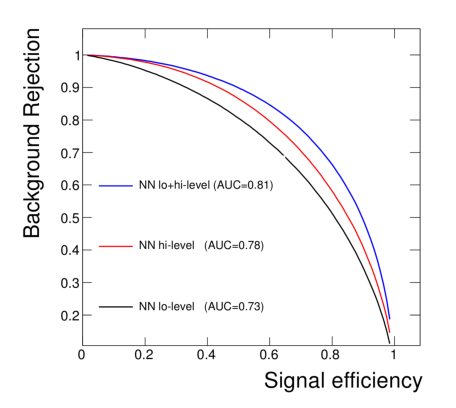
\includegraphics[width=\textwidth]{deep_a.pdf}
    \label{fig:sub1}
  \end{subfigure}%
  \begin{subfigure}{.5\textwidth}
    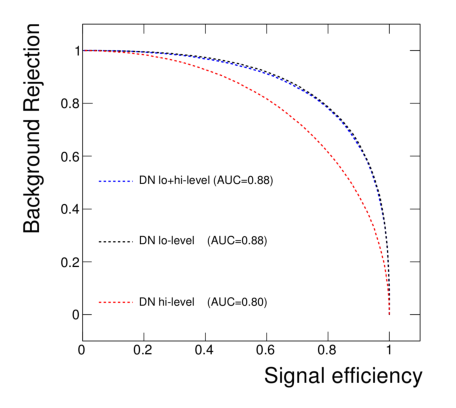
\includegraphics[width=\textwidth]{deep_b.pdf}
    \label{fig:sub2}
  \end{subfigure}
  \caption{Pouvoir de discrimination d'un réseau de neurone standard
    (gauche) et d'un réseau profond (droite). Le réseau standard a besoin des variables de haut niveau pour obtenir une performance optimale, mais pas le réseau profond. Figure tirée de la
référence~\cite{baldi_searching_2014}.}
  \label{fig:deep}
\end{figure}



%%% Local Variables:
%%% mode: latex
%%% TeX-master: "memoire"
%%% End:
